% This file was created by matlab2tikz.
%
%The latest updates can be retrieved from
%  http://www.mathworks.com/matlabcentral/fileexchange/22022-matlab2tikz-matlab2tikz
%where you can also make suggestions and rate matlab2tikz.
%

\pgfplotsset{compat=newest}

\usetikzlibrary{calc}

%%% START MACRO FOR ANNOTATION OF TRIANGLE WITH SLOPE %%%.
\newcommand{\logLogSlopeTriangle}[5]
{
	% #1. Relative offset in x direction.
	% #2. Width in x direction, so xA-xB.
	% #3. Relative offset in y direction.
	% #4. Slope d(y)/d(log10(x)).
	% #5. Plot options.
	
	\pgfplotsextra
	{
		\pgfkeysgetvalue{/pgfplots/xmin}{\xmin}
		\pgfkeysgetvalue{/pgfplots/xmax}{\xmax}
		\pgfkeysgetvalue{/pgfplots/ymin}{\ymin}
		\pgfkeysgetvalue{/pgfplots/ymax}{\ymax}
		
		% Calculate auxilliary quantities, in relative sense.
		\pgfmathsetmacro{\xArel}{#1}
		\pgfmathsetmacro{\yArel}{#3}
		\pgfmathsetmacro{\xBrel}{#1-#2}
		\pgfmathsetmacro{\yBrel}{\yArel}
		\pgfmathsetmacro{\xCrel}{\xArel}
		%\pgfmathsetmacro{\yCrel}{ln(\yC/exp(\ymin))/ln(exp(\ymax)/exp(\ymin))} % REPLACE THIS EXPRESSION WITH AN EXPRESSION INDEPENDENT OF \yC TO PREVENT THE 'DIMENSION TOO LARGE' ERROR.
		
		\pgfmathsetmacro{\lnxB}{\xmin*(1-(#1-#2))+\xmax*(#1-#2)} % in [xmin,xmax].
		\pgfmathsetmacro{\lnxA}{\xmin*(1-#1)+\xmax*#1} % in [xmin,xmax].
		\pgfmathsetmacro{\lnyA}{\ymin*(1-#3)+\ymax*#3} % in [ymin,ymax].
		\pgfmathsetmacro{\lnyC}{\lnyA+#4*(\lnxA-\lnxB)}
		\pgfmathsetmacro{\yCrel}{\lnyC-\ymin)/(\ymax-\ymin)} % THE IMPROVED EXPRESSION WITHOUT 'DIMENSION TOO LARGE' ERROR.
		
		% Define coordinates for \draw. MIND THE 'rel axis cs' as opposed to the 'axis cs'.
		\coordinate (A) at (rel axis cs:\xArel,\yArel);
		\coordinate (B) at (rel axis cs:\xBrel,\yBrel);
		\coordinate (C) at (rel axis cs:\xCrel,\yCrel);
		
		% Draw slope triangle.
		\draw[#5]   (A)-- node[pos=0.5,anchor=south] {\scriptsize 1}
		(B)-- 
		(C)-- node[pos=0.5,anchor=west] {\scriptsize #4}
		cycle;
	}
}
%%% END MACRO FOR ANNOTATION OF TRIANGLE WITH SLOPE %%%.


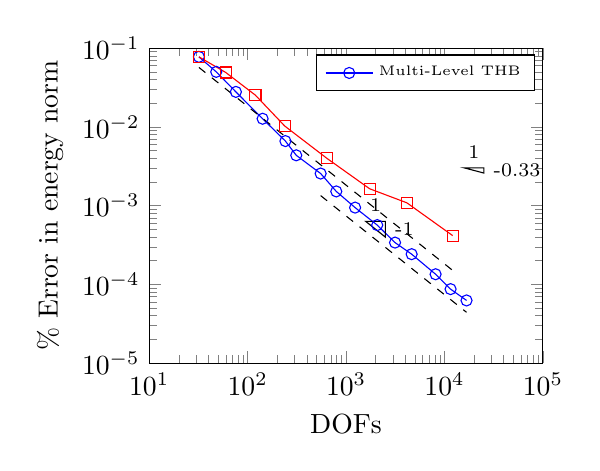
\begin{tikzpicture}

\begin{axis}[%
width=5cm,
height=4cm,
at={(0.758in,0.481in)},
scale only axis,
xmode=log,
xmin=10,
xmax=100000,
xminorticks=true,
ymode=log,
ymin=1e-05,
ymax=0.1,
yminorticks=true,
axis background/.style={fill=white},
ylabel=\% Error in energy norm,
xlabel=DOFs,
legend style={font=\tiny}
]
\addplot [color=blue,solid,mark=o,mark options={solid}]
table[row sep=crcr]{%
	32	0.0775733997153093\\
	48	0.0500073829665119\\
	76	0.0278449560820008\\
	142	0.0126970619240542\\
	242	0.00660733441696399\\
	312	0.00435668459205658\\
	552	0.00255759420607355\\
	796	0.00151589672287713\\
	1236	0.000944445092205633\\
	2074	0.000566215208140263\\
	3146	0.000339514546405781\\
	4640	0.000241941547691511\\
	8126	0.000134548935705695\\
	11536	8.70810027272917e-05\\
	16760	6.25408392329503e-05\\
};
\addplot [color=black,dashed,forget plot]
table[row sep=crcr]{%
%	32	0.0231505693963037\\
%	48	0.0154337129308691\\
%	76	0.00974760816686471\\
%	142	0.00521702972311069\\
%	242	0.0030612323168666\\
%	312	0.00237441737397987\\
	552	0.00134206199398862\\
	796	0.000930676156635324\\
	1236	0.000599367492460937\\
	2074	0.000357192970434772\\
	3146	0.000235479408989739\\
	4640	0.000159659099284853\\
	8126	9.11664066800047e-05\\
	11536	6.42179456208147e-05\\
	16760	4.42015644798161e-05\\
};

\addplot [color=red,solid,mark=square,mark options={solid},forget plot]
table[row sep=crcr]{%
	32	0.0775733997153093\\
	60	0.0490924874102604\\
	120	0.0252806230041732\\
	238	0.0102719556498042\\
	640	0.00398339340034028\\
	1736	0.00163861890120138\\
	4148	0.00108645379721495\\
	12100	0.000416598705667667\\
};
\addplot [color=black,dashed,forget plot]
table[row sep=crcr]{%
	32	0.0569412125122034\\
	60	0.0303686466731751\\
	120	0.0151843233365876\\
	238	0.00765596134617861\\
	640	0.00284706062561017\\
	1736	0.00104960760391158\\
	4148	0.000439276470682379\\
	12100	0.000150588330610786\\
};


\legend{Multi-Level THB, Tensor Product Refinement}

{
\logLogSlopeTriangle{0.6}{0.05}{0.45}{-1}{black};
\logLogSlopeTriangle{0.85}{0.05}{0.62}{-0.33}{black};
}
\end{axis}
\end{tikzpicture}%